\chapter{State of the Art} % (fold)
\label{cha:stateoftheart}

\setlength{\epigraphwidth}{11cm}
\renewcommand{\tabcolsep}{0em}

\epigraph{
\begin{tabular}{p{2.5cm}p{8.4cm}}
  \footnotesize{\textbf{\textsc{Don Draper}} :}
    & Well, technology is a glittering lure.\\
    & But there is a rare occasion when the public can be engaged on a level beyond flash ---if they have a sentimental bond with the product.\\
    & My first job I was in house at a fur company, with this old pro of a copywriter, a Greek, named Teddy. Teddy told me the most important idea in advertising is \emph{new}. It creates an itch. You simply put your product in there as a kind of calamine lotion.\\
    & He also talked about a deeper bond with a product: \emph{nostalgia}. It's delicate, but potent. Sweetheart.\\
    & \footnotesize{\emph{[starts slide show featuring photos of Draper's family.]}}\\
    & Teddy told me that in Greek, nostalgia literally means the pain from an old wound. It's a twinge in your heart, far more powerful than memory alone.\\
    & This device isn't a space ship, it's a time machine. It goes backwards, forwards. It takes us to a place where we ache to go again. It's not called a wheel, it's called a carousel.\\
    & It lets us travel the way a child travels. Round and a round, and back home again.\\
    & To a place where we know we are loved. \\
\end{tabular}
\vspace{1em}
}{\textit{The Wheel}\\ \textsc{Mad Men}}

\newpage

\section{Existing System: \idx{ScaleNet}} % (fold)
\label{sec:scalenet}

\idx{ScaleNet} \cite{SIE06} is a research project developed between 2005 and 2009.
Partly sponsored by the \emph{German Ministry of Education}, several major corporations participated, including \emph{Deutsche Telekom AG}, \emph{Alcatel SEL AG}, \emph{Eriksson GmbH}, \emph{Lucent Technologies} and \emph{Siemens AG}.
\ida{T-Labs} was specifically one of the departments more closely involved.

\begin{wrapfigure}{r}{0.5\textwidth}
  \centering
    
\includegraphics[width=0.48\textwidth]{logo-scalenet}
  \caption{\idx{ScaleNet} logo}
  \label{fig:logo-scalenet}
\end{wrapfigure}

The aim of \idx{ScaleNet} is to provide a \ida{NGN} that integrates different wireless and wireline access technologies.
It is advertised as a scalable, cost effective and efficient \ida{FMC} solution.

\subsection{System Overview} % (fold)
\label{sub:overviewscalenet}

\idx{ScaleNet} addresses both service and network convergence.
At the lower level, the system supports a multitude of heterogeneous physical and logical network elements of fixed and mobile networks into one single all-IP infrastructure.
Figure~\ref{fig:scalenet-structure} lists some of the protocols that could be used \cite{SIV08}.

\begin{figure}[htbp]
  \centering
    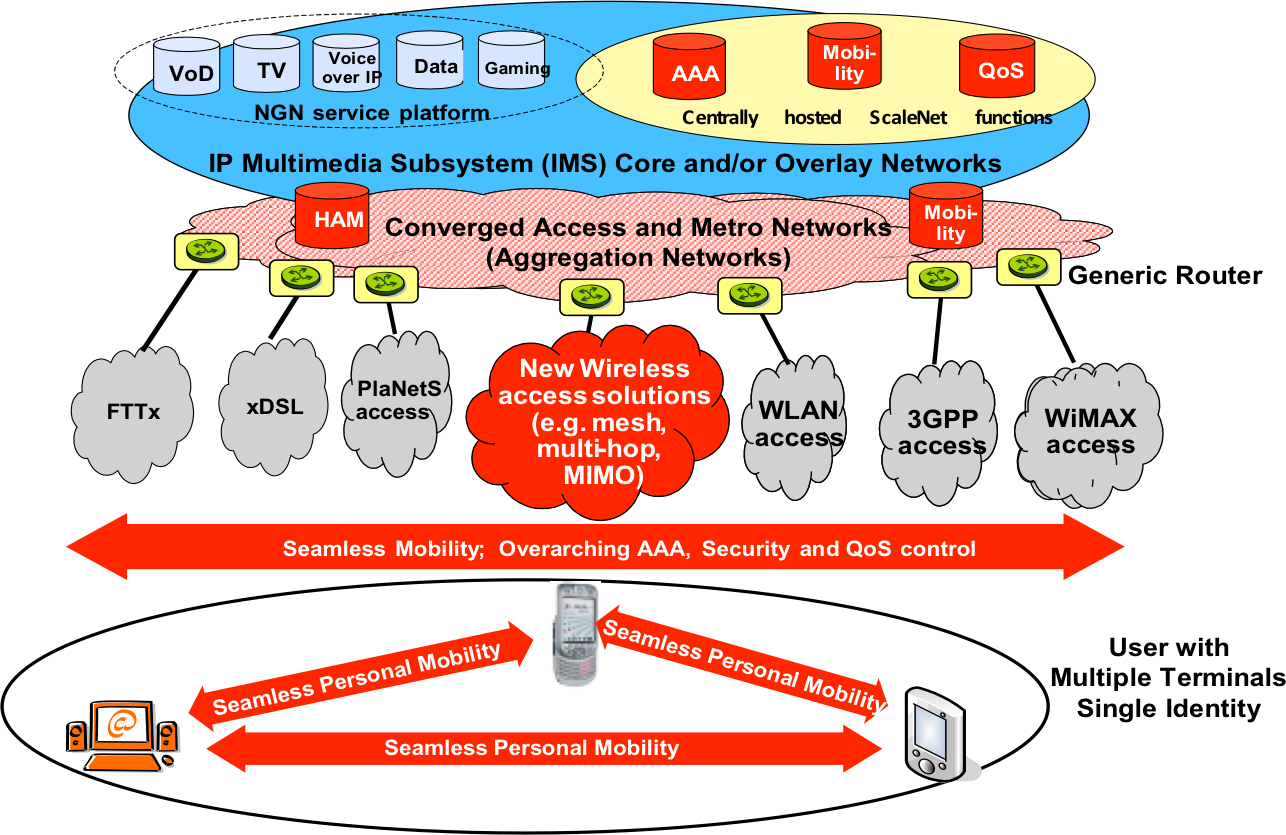
\includegraphics[width=\textwidth]{scalenet-structure}
  \caption{Structure of the system}
  \label{fig:scalenet-structure}
\end{figure}

At a upper level, multimedia services relay on the \ida{IMS} framework for the delivery.
Theoretically \idx{ScaleNet} could support other protocols like Overlay Networks or \ida{P2P}, but \ida{IMS} is the one used by the current implementation.

It is important to notice that the own network is user-centric, and transparently handles identities by using \ida{SIP}.
This eases handling users with multiple devices; therefore applications do not have to worry about that part.

It is also important to define what a session means in this system.
A session refers to the current use of a service, so for every service that the user is enjoying a session is created.
For example, if it is viewing a movie but also talking on the \ida{IP} phone, there are two sessions at the same time.

The creation of a session implies that a new service is created, but it goes the other way around too.
If a session is deleted, that service must stop.
If the user ends the service, the session must be deleted.
That means sessions have to be synchronized with the actual services.

A session is also linked to the device that the user is using.
The system allows the copy and transfer of sessions to other devices that he owns, wherever it makes sense.
Since the current implementation has also basic social capabilities, that session can also be transferred or copied to a user's contact.
In the context of this application a user's contact is called ``buddy''.
Figure~\ref{fig:scalenet-structure} lists some of the services that can be offered:

\begin{itemize}
  \item Voice \et{} Video Calls
  \item Mobile TV \et{} \ida{VOD}
  \item \index{MMOG}\acp{MMOG}
  \item Internet Access
\end{itemize}

The work described in this document is primarily focused on the second application, i.e., video streaming.
The idea is that the user can buy a video and play it anywhere using any supported device.

\nicesubsectionending

% subsection overviewscalenet (end)

\subsection{\idx{IMS} Demonstrator} % (fold)
\label{sub:demonstrator}

\begin{figure}[p]
  \centering
    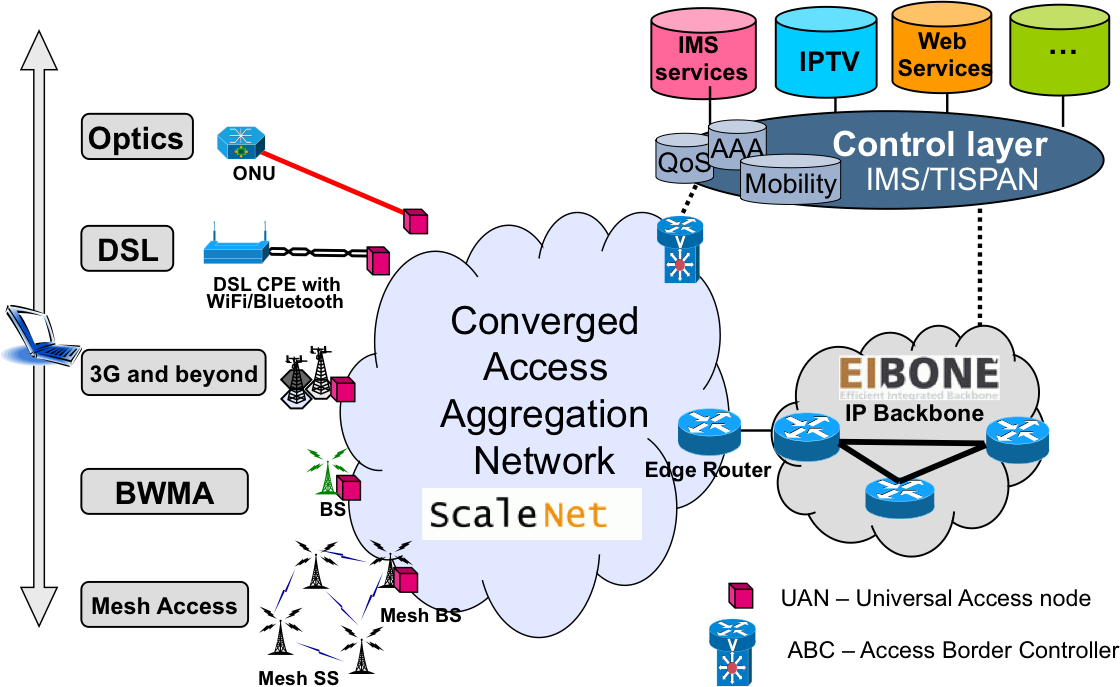
\includegraphics[width=\textwidth]{ims-arch}
  \caption{System architecture}
  \label{fig:ims-arch}
\end{figure}

\begin{figure}[p]
  \centering
    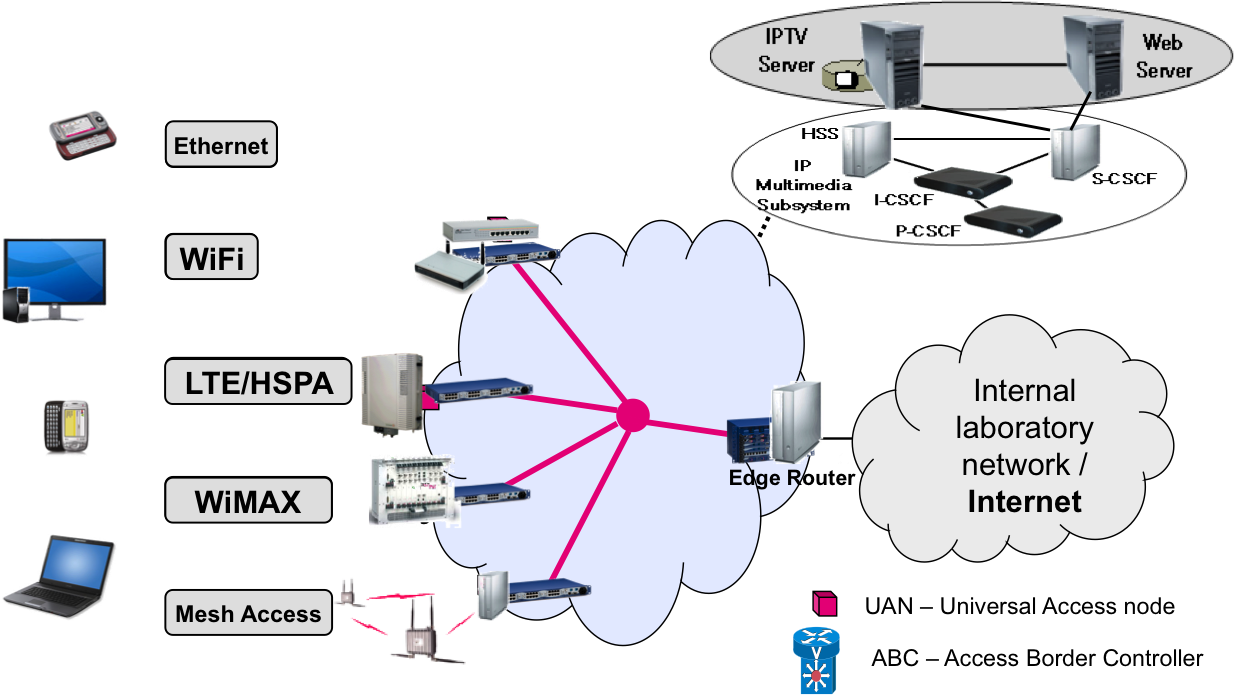
\includegraphics[width=\textwidth]{ims-arch-real}
  \caption{Architecture of the demonstrator}
  \label{fig:ims-arch-real}
\end{figure}

A logical view of the system is depicted in Figure~\ref{fig:ims-arch}, explaining the important nodes based on the capabilities needed.
The information relevant to this project is contained in the upper right corner of the figure, the nodes behind the control layer.

In the offices of \ida{T-Labs} in Berlin and Darmstadt there is a demonstrator with a working implementation of \idx{ScaleNet}.
That demonstrator is composed by several servers and a network infrastructure that enables access to the system using different network protocols and devices.
In Figure~\ref{fig:ims-arch-real} the actual network and hardware are exposed, replacing the same space as in the logical view (Figure~\ref{fig:ims-arch}).

\begin{figure}[htbp]
  \centering
    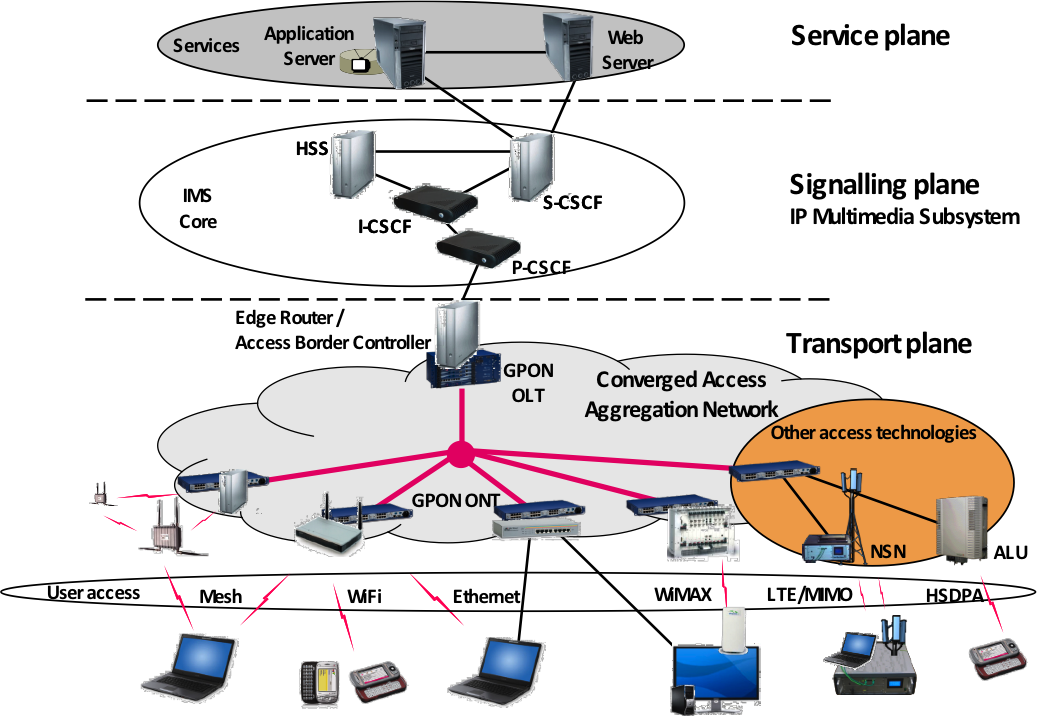
\includegraphics[width=\textwidth]{ims-setup}
  \caption{Setup of the demonstrator}
  \label{fig:ims-setup}
\end{figure}

Figure~\ref{fig:ims-setup} describes the setup in a better way and highlights the three different planes of the demonstrator.
The developed web application is executed from the \idx{Web Server} and the \idx{Application Server}, since it belongs to the service plane.
The signaling plane has also to be taken into account, because it communicates directly with the servers.

However, that is not the real deployment of the hardware used.
Whether for convenience or efficiency, tasks are distributed between two main servers.
This does not affect the logic of the system, since those tasks could be easily decoupled in an alternate deployment with more servers.
Anyway, the interesting pieces of hardware for this project are:

\begin{description}
  \item[\ida{IMS} core] This machine contains the \ida{IMS} server\footnote{The IMS core is open source software from Fraunhofer FOKUS and it can be freely downloaded from: \url{http://www.openimscore.org/}}, but since the \ida{IMS} load is not very high, it is responsible for other things.
  It acts as a \idx{Web Server} (using Apache Web Server\footnote{\url{http://httpd.apache.org/}}) serving \idas{PHP} applications.
  It is also the internal \idas{DNS} server.
  \item[\idx{Application Server}] This is the \idas{IPTV} server, where the video content is streamed.
  It is also a \idx{Web Server}, but it serves \idx{Java} applications based on the \idas{OSGi} framework\footnote{\url{http://www.osgi.org/}}.
  \item[User Devices] Devices intended for the user to access the services.
  There is a TV, a laptop and several phones.
  All of them run a custom \ida{IMS} client that holds a connection to the servers, allowing the identification and adding \idas{IPTV} and \idas{VoIP} capabilities to those devices.
  In the last phase of the development, an \idx{iPhone} was added for testing purposes.
\end{description}

This demonstrator contains several demo applications running.
The interesting one for this project is the application that handles \idas{IPTV} streaming.

\nicesubsectionending

% subsubsection stoppingplayback (end)

\subsection{Personal Network Administration Interface (\idx{PNAI})} % (fold)
\label{sub:pnai}

The Web interface used for the management of sessions is called \ida{PNAI}. From this interface the user can obtain this information:

\begin{itemize}
  \item All devices and registered in the system for that user and their online status.
  \item All buddies for that user and their online status.
  \item All multimedia sessions related to the user. This includes:
  \begin{itemize}
    \item The sessions running on his devices, no matter who paid for that content.
    \item The sessions running on devices from his buddies and started/paid by that user.
  \end{itemize}
\end{itemize}

Those are passive actions, but from that same view the user can initiate some operations to control the system.
In Figure~\ref{fig:usecasesiptv} all the available operations relating sessions are listed following a use case diagram.

\begin{figure}[htbp]
  \centering
    \includegraphics[width=\textwidth]{diagrams/usecases.1}
  \caption{Use cases for the IPTV application}
  \label{fig:usecasesiptv}
\end{figure}

In that diagram colors are used to differentiate the different kind of use cases covered. Also two visual marks (* and **) are added in case this is a copy in black a white. The meaning of the colors are explained according to this legend:

\begin{description}
  \item[Green] Available already in the main \ida{PNAI} page.
  \item[Purple (\emph{marked with *})] Available in an individual page outside of the main \ida{PNAI} page.
  \item[Red (\emph{marked with **})] Not implemented.
\end{description}

As we can see, the main \ida{PNAI} page has already a lot of functionality, but it can contain even more. Basically the actions available to that user in that page are:

\begin{itemize}
  \item Terminate a session of a user device or of a buddy if the session is owned by that user.
  \item Transfer (handover) or copy (duplication) a existing session to a user device or to a buddy if the session is owned by that user. That is, if one buddy bought the content for us, we cannot transfer again that content to another buddy.
\end{itemize}

Beside of these session related operations, there are other management operations.
For example, selecting which device is the default, adding/removing devices or adding/removing buddies.
For this document they are not relevant since they remained untouched.

Figure~\ref{fig:pnai-old} shows the old appearance of the main page for a logged user, before any work began.
On the left side of the page there is the \idx{Device List}, where the devices owned by that user are drawn.
On the right side there is the \idx{Buddy List}, where the user's buddies are listed.
Finally, the trash is in the lower right corner of the \idx{Device List}. 

\begin{figure}[htbp]
  \centering
    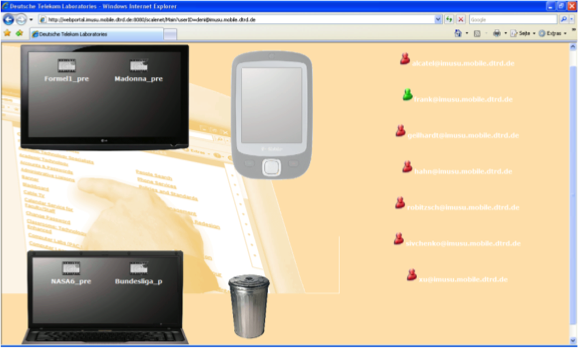
\includegraphics[width=\textwidth]{pnai-old}
  \caption{Old main \idas{PNAI} page}
  \label{fig:pnai-old}
\end{figure}

The devices that are offline are disabled and are drawn with a whitish appearance.
The buddies that are online are preceded by a green icon, while the ones that are offline are preceded by a red icon.

Devices or buddies that are online act as session containers. Inside of the 

\subsubsection{Use Cases} % (fold)
\label{ssub:usecasesold}

\begin{center}
  \begin{usecase}[Stop a session of a device]
    \label{tab:usecasestopdevice}%
    \usecaseactor{System user}
    \usecasepre{A session is already running on a device, and it is showing in the \ida{PNAI} interface inside of that device.}
    \usecasepost{Session must terminate, i.e., the content must stop playing. The user must be notified with a popup and the session icon must be deleted from the \ida{PNAI} interface.}
    \usecasemain{
      \begin{usecasepath}
        \item User starts dragging the session icon.
        \item A copy of the session icon appears under the user's cursor, and follows the cursor until the user drops it.
        \item User drops the cloned session icon into the trash.
        \item A popup appears to notify the user that the action is in progress and the cloned session icon is deleted from the view.
        \item The content stops playing.
        \item The popup disappears and the original session icon is deleted from the view.
      \end{usecasepath}
    }
    \usecasealt{1}{
      \begin{usecasepath}[b]
        \setcounter{enumi}{2}
        \item User drops the session into a blank space.
        \item Action is cancelled.
      \end{usecasepath}
    }
    \usecasealt{2}{
      \begin{usecasepath}[c]
        \setcounter{enumi}{4}
        \item There is an error with the server and the content keeps playing.
        \item The content of the popup changes to notify the user that there was an error with the server and the action could not be completed.
        After 5 seconds it disappears.
        \item Action is cancelled.
      \end{usecasepath}
    }
    \usecasealt{3}{
      \begin{usecasepath}[d]
        \item There is an error with the server and the content keeps playing.
        \item The content of the popup changes to notify the user that there was an error with the server and the action could not be completed.
        After 5 seconds it disappears.
        \item Action is cancelled.
      \end{usecasepath}
    }
  \end{usecase}
\end{center}

The use case for terminating a session that a buddy is playing and that we own is very similar:

\begin{center}
  \begin{usecase}[Stop a session of a buddy]
    \label{tab:usecasestopbuddy}%
    \usecaseactor{System user}
    \usecasepre{A session owned by the user is running on a device, and it is showing in the \ida{PNAI} interface near that buddy's name.}
    \usecasepost{Session must terminate, i.e., the content must stop playing. The user must be notified with a popup and the session icon must be deleted from the \ida{PNAI} interface. The buddy is \emph{not} notified, the content stops without warning.}
    \usecasemain{
      \begin{usecasepath}
        \item User starts dragging the session icon.
        \item A copy of the session icon appears under the user's cursor, and follows the cursor until the user drops it.
        \item User drops the cloned session icon into the trash.
        \item A popup appears to notify the user that the action is in progress and the cloned session icon is deleted from the view.
        \item The content stops playing.
        \item The popup disappears and the original session icon is deleted from the view.
      \end{usecasepath}
    }
    \usecasealt{1}{
      \begin{usecasepath}[b]
        \setcounter{enumi}{2}
        \item User drops the session into a blank space.
        \item Action is cancelled.
      \end{usecasepath}
    }
    \usecasealt{2}{
      \begin{usecasepath}[c]
        \setcounter{enumi}{4}
        \item There is an error with the server and the content keeps playing.
        \item The content of the popup changes to notify the user that there was an error with the server and the action could not be completed.
        After 5 seconds it disappears.
        \item Action is cancelled.
      \end{usecasepath}
    }
  \end{usecase}
\end{center}

% subsubsection usecasesold (end)


% subsection pnai (end)

% section scalenet (end)

\section{Server Programming Language: \idx{PHP}} % (fold)
\label{sec:php}

\ida{PHP}\footnote{\url{http://www.php.net/}} is one of the languages used to build front-end web applications in \idx{ScaleNet}, and it is one of the most popular languages for building web applications in general.
Not only most of the portal is written in this language but, eventually, the \ida{PNAI} interface will be ported from an \ida{OSGi} bundle to a \ida{PHP} script.

\subsection{History} % (fold)
\label{sub:phphistory}

Originally, \ida{PHP} was created in 1995 by \emph{Rasmus Lerdorf} as a set of \ida{CGI} scripts written in \idx{C} that parsed \ida{HTML} files.
The goal was being able to call specific \idx{C} routines and show its output when a page was visited, by directly embedding the code in the \ida{HTML} source.
In the next years this open source project became a full-fledged parser, creating a new generic language.

\begin{wrapfigure}{r}{0.5\textwidth}
  \centering
    
\includegraphics[width=0.48\textwidth]{logo-php}
  \caption{\idx{PHP} logo}
  \label{fig:logo-php}
\end{wrapfigure}

In 1997 \emph{Zeed Suraski} and \emph{Andi Gutmans} rewrote that parser to include more functionality and released it as \ida{PHP} 3.
Then, specially after \ida{PHP} 4, the language started to be widely used.
\ida{PHP} has gained a lot of popularity for web development projects and it is used in big websites like Yahoo, Facebook and Wikipedia.

In 2004 \ida{PHP} 5 was released, adding \ida{OOP} capabilities to the language.
However, it is compatible with \ida{PHP} 4 scripts, so it is optional to work in an Object-Oriented way.
This is the most recent version and it is the one installed in the \idx{IMS} demonstrator.

% subsection phphistory (end)

\subsection{Quick Overview of the Language} % (fold)
\label{sub:overviewphp}

A \ida{PHP} file is basically a \ida{HTML} file with the \texttt{.php} extension that it is usually stored in the public folder of the server (\idx{Apache}, \ida{IIS} or other supported server).
When that page is requested, the server calls the \ida{PHP} module, that parses that file and returns a normal \ida{HTML} page.

The interesting things happen within its delimiters
(usually <?php and ?>), where the \ida{PHP} code is written.
Outside of these delimiters the text is treated as a normal \ida{HTML} soup and therefore not processed.
Listing~\ref{phpexample} shows an example of \ida{PHP} code embedded within \ida{HTML} code and Listing~\ref{phpexampleafter} shows the resulting \ida{HTML} output.

\begin{lstlisting}[float=htbp,label=phpexample,language=php,alsolanguage=html,caption=\idx{PHP} code embedded within \idx{HTML} code]
  <!DOCTYPE html>
  <html>
    <head>
      <title>PHP Test</title>
    </head>
    <body>
    <?php
    for ($i = 0; $i < 5; $i++) {
      echo "<p>Hello World " . $i . "</p>\n";
    }
    ?>
    </body>
  </html>
\end{lstlisting}

\begin{lstlisting}[float=htbp,label=phpexampleafter,language=html,caption=Resulting \idx{HTML} code]
  <!DOCTYPE html>
  <html>
    <head>
      <title>PHP Test</title>
    </head>
    <body>
    <p>Hello World 0</p>
    <p>Hello World 1</p>
    <p>Hello World 2</p>
    <p>Hello World 3</p>
    <p>Hello World 4</p>
    </body>
  </html>
\end{lstlisting}

Its syntax is very similar to \idx{C}, with equivalent constructions (if conditions, for and while loop, functions, etc).
Some notable exceptions are that variables must start with a dollar sign character (\texttt{\$}), and that a dot is used for concatenating strings instead of the most traditional plus sign.

Variables are dynamically typed, so the programmer does not need to specify types. A variable's type is determined by the context in which that variable is used, so any variable can hold different types during an execution.

One of the strengths of \ida{PHP} is the wide range of utility functions bundled in the processor and in additional extensions usually included in distributions.
Although objects are supported in \ida{PHP} 5, it is not discussed here because the scripts in \idx{ScaleNet} do not use them.

Global variables like \idc{\$\_GET}, \idc{\$\_POST} or \idc{\$\_SERVER} offer access to information sent from the browser, so it is commonly used to pass parameters to a \ida{PHP} script (through the \ida{URL} or forms in the page).
On the other hand \idc{\$\_SESSION} and \idc{\$\_COOKIE} allow to store some data through the same \emph{visit}, even across different scripts.

Since the main goal of the language is generating \ida{HTML} content, the most common functions are ones that \emph{print} text in the output, like \idc{echo}.
Because \idx{MySQL} is quite popular in web development, there is an extension with functions to interact with those databases.

Other commons functions are \idc{include} (to, ehem, include other \ida{PHP} source files), \idc{isset} (to know is a variable is set), \idc{die} (to terminate the execution of the script at any moment), \idc{header} (to set \idc{HTTP} headers) and diverse string/array manipulation functions.

% subsection overviewphp (end)

% section php (end)
\section{Server Programming Language: \idx{Java}} % (fold)
\label{sec:java}

Lorem ipsum dolor sit amet, consectetur adipisicing elit, sed do eiusmod tempor incididunt ut labore et dolore magna aliqua. Ut enim ad minim veniam, quis nostrud exercitation ullamco laboris nisi ut aliquip ex ea commodo consequat. Duis aute irure dolor in reprehenderit in voluptate velit esse cillum dolore eu fugiat nulla pariatur. Excepteur sint occaecat cupidatat non proident, sunt in culpa qui officia deserunt mollit anim id est laborum.

\subsection{Quick Overview of the Language} % (fold)
\label{sub:overviewjava}

Lorem ipsum dolor sit amet, consectetur adipisicing elit, sed do eiusmod tempor incididunt ut labore et dolore magna aliqua. Ut enim ad minim veniam, quis nostrud exercitation ullamco laboris nisi ut aliquip ex ea commodo consequat. Duis aute irure dolor in reprehenderit in voluptate velit esse cillum dolore eu fugiat nulla pariatur. Excepteur sint occaecat cupidatat non proident, sunt in culpa qui officia deserunt mollit anim id est laborum.

% subsection overviewjava (end)

\subsection{OSGI} % (fold)
\label{sec:osgi}

Lorem ipsum dolor sit amet, consectetur adipisicing elit, sed do eiusmod tempor incididunt ut labore et dolore magna aliqua. Ut enim ad minim veniam, quis nostrud exercitation ullamco laboris nisi ut aliquip ex ea commodo consequat. Duis aute irure dolor in reprehenderit in voluptate velit esse cillum dolore eu fugiat nulla pariatur. Excepteur sint occaecat cupidatat non proident, sunt in culpa qui officia deserunt mollit anim id est laborum.

% subsection osgi (end)

\subsection{Java Applets} % (fold)
\label{sub:javaapplets}

Lorem ipsum dolor sit amet, consectetur adipisicing elit, sed do eiusmod tempor incididunt ut labore et dolore magna aliqua. Ut enim ad minim veniam, quis nostrud exercitation ullamco laboris nisi ut aliquip ex ea commodo consequat. Duis aute irure dolor in reprehenderit in voluptate velit esse cillum dolore eu fugiat nulla pariatur. Excepteur sint occaecat cupidatat non proident, sunt in culpa qui officia deserunt mollit anim id est laborum.

% subsection javaapplets (end)

% section java (end)

\section{Interface: \idx{HTML} and \idx{CSS}} % (fold)
\label{sec:htmlcss}

Lorem ipsum dolor sit amet, consectetur adipisicing elit, sed do eiusmod tempor incididunt ut labore et dolore magna aliqua. Ut enim ad minim veniam, quis nostrud exercitation ullamco laboris nisi ut aliquip ex ea commodo consequat. Duis aute irure dolor in reprehenderit in voluptate velit esse cillum dolore eu fugiat nulla pariatur. Excepteur sint occaecat cupidatat non proident, sunt in culpa qui officia deserunt mollit anim id est laborum.

\subsection{HTML} % (fold)
\label{sub:html}

Lorem ipsum dolor sit amet, consectetur adipisicing elit, sed do eiusmod tempor incididunt ut labore et dolore magna aliqua. Ut enim ad minim veniam, quis nostrud exercitation ullamco laboris nisi ut aliquip ex ea commodo consequat. Duis aute irure dolor in reprehenderit in voluptate velit esse cillum dolore eu fugiat nulla pariatur. Excepteur sint occaecat cupidatat non proident, sunt in culpa qui officia deserunt mollit anim id est laborum.

% subsection html (end)

\subsection{CSS} % (fold)
\label{sub:css}

Lorem ipsum dolor sit amet, consectetur adipisicing elit, sed do eiusmod tempor incididunt ut labore et dolore magna aliqua. Ut enim ad minim veniam, quis nostrud exercitation ullamco laboris nisi ut aliquip ex ea commodo consequat. Duis aute irure dolor in reprehenderit in voluptate velit esse cillum dolore eu fugiat nulla pariatur. Excepteur sint occaecat cupidatat non proident, sunt in culpa qui officia deserunt mollit anim id est laborum.

% subsection css (end)

\subsection{HTML5 and CSS3} % (fold)
\label{sub:html5css3}

Lorem ipsum dolor sit amet, consectetur adipisicing elit, sed do eiusmod tempor incididunt ut labore et dolore magna aliqua. Ut enim ad minim veniam, quis nostrud exercitation ullamco laboris nisi ut aliquip ex ea commodo consequat. Duis aute irure dolor in reprehenderit in voluptate velit esse cillum dolore eu fugiat nulla pariatur. Excepteur sint occaecat cupidatat non proident, sunt in culpa qui officia deserunt mollit anim id est laborum.

% subsection html5css3 (end)

% section htmlcss (end)
\section{Client Programming Language: \idx{JavaScript}} % (fold)
\label{sec:javascript}

The only programming language available natively in browsers is \idx{JavaScript}, so any modern interactive web application should embrace it.
Given that the web has become such a popular platform and \idx{JavaScript} has a steep learning curve, the language is getting more attention lately and all indications point to a very bright future.
Most of the coding in this project was done in \idx{JavaScript}.

\subsection{History} % (fold)
\label{sub:jshistory}

\emph{Brendan Eich} originally developed the \idx{JavaScript} language working at \emph{Netscape Corp.} under the name of \emph{Mocha}, renamed to \emph{LiveScript} and then again to finally \idx{JavaScript}.

First implemented in \idx{Netscape} Navigator 2.0 in 1995, and contrary to whatever the name may lead to think, it has little to none to do with \idx{Java}.
Indeed, the name only served more marketing purposes.
The competitor, Microsoft, added support for the essentially the same language in \ida{IE} 3 the next year, but called \emph{JScript} to avoid trademark issues.

\begin{wrapfigure}{r}{0.5\textwidth}
  \centering
    
\includegraphics[width=0.48\textwidth]{logo-javascript}
  \caption[JavaScript logo]{Since there is no official \idx{JavaScript} logo, here is a rhino}
  \label{fig:javascript-logo}
\end{wrapfigure}

Then \idx{Netscape} delivered the language to the \ida{ECMA} for standardization.
The effort culminated in 1997 with the first edition of a new open standard called \emph{ECMAScript}, named as a compromise in the dispute between Netscape and Microsoft.
For some reason, that name was never popularized, instead the original term \idx{JavaScript} is used in almost every situation.

Being closely linked with a markup language that even non-programmers and \emph{amateurs} could code, \idx{JavaScript} was initially disregarded as a toy by many traditional developers.
Other apparent limitations of the language, a very lenient parser, performance issues and compatibility problems between browsers did not help its popularity either.

However, the advent of \ida{AJAX}, its ubiquity in browsers, better/faster parsers and the need for more complex web interfaces put \idx{JavaScript} back in every professional web developer toolbox.
Since then a multitude of framework and libraries have been released to ease the development, with its usage growing broadly not only in browsers but even in server applications.

% subsection jshistory (end)
\subsection{Quick Overview of the Language} % (fold)
\label{sub:overviewjavascript}

At first glance the syntax may seem a simplified version of \idx{Java} (or other C-based language), but much more direct (no classes, packages, etc.).
Make no mistake, under the hood \idx{JavaScript} hides a lot of powerful constructions that makes it flexible enough to suit diametrical programming paradigms.
Some of the most important features are:

\begin{description}
  \item[Scripted] The browser receives the plain source code, and then it is interpreted and run.
  The big advantage is that it does not needed to be compiled beforehand, the traditional disadvantage is that it is slower than native code or even \idx{Java} byte code.
  
  Nevertheless, a lot of improvements have been deployed lately in browser engines, and new techniques like \ida{JIT} nearly close that gap.
  On the other hand, similarly to other script-based languages, it is easy to end up with a low-quality codebase, since inexperienced programmers can quickly write working code.
  \item[Imperative statements] It supports the basic imperative paradigm with the typical if statements, while and for loops, global functions, etc.
  It is not required to think about objects to make a script, with those things it can be possible to write a full-fledged application if wanted.
  \item[Object based] Internally, in \idx{JavaScript} everything is an object, not only variables but even functions or undefined values.
  However, there are no classes like in \idx{Java}, to create a new object it can be specified in a literal notation or using a constructor (a plain function).
  \item[Prototype based] The language is classless, but inheritance between objects is possible through the use of \emph{prototypes}.
  A prototype is just an object used as a template from which to get the initial properties for a new object.
  If an object is asked for a property (also known as \emph{attributes} and \emph{methods} in \idx{Java} jargon) it does not have, its parent is asked, and then again until the property is found or until the root object is found (the end of the \emph{chain}).
  Listings~\vref{oopjs} and \vref{oopjava} show how inheritance works in \idx{JavaScript} compared to \idx{Java}.
  
\begin{lstlisting}[float=htbp,label=oopjs,language=javascript,caption=Inheritance in JavaScript]
  function Employee() {
    this.name = "";
    this.dept = "general";
    this.hello = function() {
      console.log("Hello, I'm " + this.name);
    };
  }
  function Engineer() {
    this.dept = "engineering";
    this.projects = [];
  }
  Engineer.prototype = new Employee;

  var john = new Engineer();
  john.name = "John Doe";
  john.hello();
\end{lstlisting}

\begin{lstlisting}[float=htbp,label=oopjava,language=java,caption=Inheritance in Java]
  public class Employee {
    public String name;
    public String dept;
    public Employee() {
      this.name = "";
      this.dept = "general";
    }
    public void hello() {
      System.out.println("Hello, I'm " + this.name);
    }
  }
  public class Engineer extends Employee {
    public String[] projects;
    public Engineer() {
      this.dept = "engineering";
      this.projects = new String[0];
    }
  }
  Employee john = new Engineer();
  john.name = "John Doe";
  john.hello();
\end{lstlisting}
  
  It is easy to demonstrate that this abstraction can be more powerful than classes because a similar class-based \ida{OOP} behavior can be achieved with prototypes but the opposite is not true.
  \item[First-class functions] As said before, \idx{JavaScript} functions are objects, so they have properties and methods and can be assigned to variables as every other object.
  Moreover, these functions can be passed as arguments, returned as other function values and invoked in any moment and scope using multiples ways (such as the \verb+()+ operator).
  
  Functions do not need to be defined in the global scope, they can be defined inside other functions.
  Nowadays the use of closures (specifically anonymous functions) is considered a very good practice to avoid cluttering the global scope with variables.
\end{description}

As stated repeatedly, every variable in \idx{JavaScript} contains a reference to an object.
However, that does not mean that values do not have a type, and there are several primitive types available in the language.
In any case, even literals of these types have accessible properties like any other object.

\begin{description}
  \item[Undefined and Null] Before assigning some value, a variable holds the value \idc{undefined}.
  This \idc{undefined} is the only object of, pun intended, type \idc{undefined}, a full-fledged object that can be even used in assignments.
  On the other hand, \idc{null} is never used by \idx{JavaScript}, so if some variable holds this value, it must have been set programmatically by the developer.
  Although the type \idc{null} is apparently \idx{Object}, internally it is also the only value of type \idc{null}.
  \item[Number] In \idx{JavaScript} there is no external distinction between integers, floating point values and others, every literal number is treated equally and has the same properties.
  Internally they are all doubles, floating points numbers with an accuracy nearly 16 significant digits, so some real numbers cannot be represented.
  \item[String] Strings are delimited by double quotes and single quotes indistinctly, the only difference is which quotes need to be escaped inside of the string.
  \item[Boolean] As usual, there are only two values possible in this data type: \texttt{true} or \texttt{false}.
\end{description}

For all of these types (except undefined/null), there are object constructors, but the preferred way to initialize them is through plain literals.
Besides these primitives data types, there are also several native objects built in the language:

\begin{description}
  \item[Array] As other C-based languages, arrays are available to store a collection of values in a variable using integers as keys.
  To create an empty literal array (also preferred to the Array constructors), two square brackets can be used.
  This bracket notation can also used for accessing object properties, so it can be confused with associative arrays while the language does not support this directly.
  \item[Date] A simple object to store and manipulate dates down to a milliseconds.
  \item[Error] Similarly to exceptions in other languages, this kind of objects can be thrown in case of error (using the throw clause) and caught for error handling (using the try/catch block).
  \item[Math] This object cannot be \emph{instantiated} and it only contains math-related constants and functions.
  \item[Regular Expression] Literals between backslashes represents regular expressions, and they hold some useful methods to deal with search and replace in strings.
  The \texttt{RegExp} constructor can be used but, again, it is not recommended.
  \item[Function] Functions are declared by using the keyword \texttt{function}, an optional name, the arguments and the body block.
  The object constructor, though also available, is very ill-advised, as it relies on strings.
  \item[Object] The rest of the values are of type \idx{Object} or indirectly inherit from this type.
  Objects literals are represented by curly brackets and a comma-separated list of keys/values separated by colons.
  This literal syntax is the base for \ida{JSON}, a notation used for data exchange that can be natively used in \idx{JavaScript}.
\end{description}

% subsection overviewjavascript (end)
\subsection{The DOM} % (fold)
\label{sub:dom}

Apart from the native capabilities of the \idx{JavaScript} language, browsers provide a very useful tool to deal with the \ida{HTML} elements of the page, the \ida{DOM}.
It consists of an \ida{API} accessible from \idx{JavaScript} and it allows the dynamic retrieval, creation, modification and deletion of \ida{HTML} elements within the page scope.

This \ida{DOM} is a fully object-oriented representation of the web page, in which every element is depicted as an object with properties that responds accordingly to different methods.
Those properties determine the document structure, style and content.
Actually, this representation is not bound to \idx{JavaScript} or even browsers, it can be accessed with other programming languages and applications.
But since \idx{JavaScript} is the most popular one in browsers they are usually delineated as partners.

The basic idea behind the \ida{DOM} is that the page is composed around a tree of elements (nodes).
Starting from the root node, every element may have an indeterminate number of children.
The \ida{DOM} provides some methods to traverse that tree either by depth (between a parent and its children) or breadth (between siblings).
Visually, children are drawn inside their parent bounds, but that behavior can be subverted with the use of \ida{CSS} properties.

This \ida{API} forms a standalone standard maintained by the \ida{W3C}.
But, as other web standards, its support varies from browser to browser, each one suffering from either partial implementations, vendor extensions or, commonly, both.

Another chronic burden is that modifying visible elements in the page is a very expensive operation.
Since the \ida{DOM} is linked to the visual representation of the page, every modification triggers a live partial or full page reflow.
For this reason it is advisable that, when several \ida{DOM} changes are needed, they are made on a detached element and, at the end, that element is attached to the \ida{DOM} tree.

\subsubsection{DOM Objects} % (fold)
\label{ssub:domobjects}

There are several objects available to \idx{JavaScript} exposed by the \ida{DOM}.
Those objects properties and functions conforms the \ida{API}.
The most important ones are:

\begin{description}
  \item[window] This object represents the browser window itself, and it allows the retrieval and modification of several properties related to the browser in general and the document window in particular.
  Since this is the global object, all of its properties are initially accessible with no need to specify \idc{window}, as if they were \emph{local variables}, so for example \idc{location} is the same as \texttt{window.location}.
  It has lots of attributes, some of the most important being:
  \begin{description}
    \item[window.location] Through this property the location (\ida{URL}) for the window can be accessed and modified.
    \item[window.innerHeight / window.innerWidth] These readonly properties contains the size of the content area of the browser window. That is, only the area occupied by the document, not counting external browser elements like the title bar, the status bar or the menu bar.
    \item[window.screen] This object describes the screen: its size, its color depth and the position of the window in the screen.
    \item[window.navigator] This object contains information about the browser, such as the user agent, browser version, platform, language, plugins installed, etc.
    Modern browsers also include access to geolocation data in this object.
    \item[window.history] This object provides an interface for manipulating the browser session history, i.e., the pages visited by the user in this tab.
    Initially it was not possible to change or read the history, only traveling through it, but an \ida{HTML}5 extension encloses several methods to add and modify history entries (but not read).
    \item[window.localStorage] This object contains the Web Storage \ida{API}, one of the key components of \ida{HTML}5.
    Basically, it simplifies the storage of significant amounts of data locally in the browser, so that it is available in successive visits using a key/value pairs interface.
    \item[window.applicationCache] Another key component of \ida{HTML}5, through this object the cache of static files is managed, allowing the rising of offline web applications.
    \item[window.setTimeout() / window.clearTimeout()] This useful function executes a function after the specified delay.
    It returns a timer identifier that allows canceling it afterwards.
    \item[window.setInterval() / window.clearInterval()] Similar to the previous function, this sets a timer that will repeatedly execute a function with a fixed time delay between calls.
    \item[window.open()] It opens an additional window with the size and properties specified.
    \item[window.close()] It closes the current window but it only works if the window was opened programmatically by \idx{JavaScript}.
    \item[window.scroll()] This function scrolls the window to a particular coordinate in the document.
    \item[window.escape() / window.unescape()] A very useful utility function to encode/decode special characters in a string so it is suitable for cookie storage or \ida{HTTP} requests.
  \end{description}
  \item[document] The interface of this object comprises all the necessary tools to retrieve and modify the document, with particularly valuable functions for \ida{DOM} retrieval.
  Therefore, it is almost impossible to make a web application without accessing this object, either directly or employing a \idx{JavaScript} library.
  The most relevant properties and methods are:
  \begin{description}
    \item[document.cookie] This object contains the interface to get and set the cookies of a page, that is, a small amount of data stored in the client that will be usually to maintain a session with the server.
    Since these cookies will be transferred with every request to the server, its overuse could slow the page loading.
    \item[document.styleSheets] This readonly object contains references to all the stylesheets in the page.
    There are also properties for accessing other kind of elements, like \texttt{document.links}, \texttt{document.images}, \texttt{document.forms}, etc, but in modern \idx{JavaScript} paradigms these are not very used anymore.
    \item[document.title] This object gets and sets the title of the document, which most browsers used for their window titles.
    \item[document.referrer] This string contains the address of the page that linked to this page.
    \item[document.getElementById()] This function returns the element with the specified id.
    It is the basic pillar of element manipulation, since it is the most used method to directly fetch an element.
    Because of that, multiple libraries have wrapped this function under the \texttt{\$()} short name.
    \item[document.getElementsByClassName()] Similar to the previous function, this one returns the elements with the given class name.
    This is natively implemented only in relatively modern browsers, but it is so obviously useful that it was already widely implemented in most third-party libraries and toolkits.
    \item[document.getElementsByTagName()] The third-wheel of the last two functions, this one returns the elements with the given tag name.
    It seems useful for dealing with all the elements of a certain type, but since \ida{DOM} manipulations are normally needed inside a certain document \emph{block} rather than across element types in all the document, its counterpart that affects only an element children is more interesting.
    \item[document.createElement()] This function returns a newly created element with the given tag name.
    This does not add the element to the document tree, it is needed to insert it manually later on.
    \item[document.createAttributeName()] This function returns a newly created attributed node with the given name.
    This function does not add the attribute to any element, it is needed to set it manually later on.
    This is not very used, since the \texttt{element.setAttributeName()} is more convenient, but it could be more efficient if the same attributes need to be changed in a lot of different elements.
    \item[document.createDocumentFragment()] This function creates a document fragment, an temporary holding object designed to store nodes before adding them to the document.
    It is not very known, but it is one of the best performance-wise solutions when several elements need to be added to the document.
    \item[document.evaluate() / document.createExpression()] These functions provide an interface to work with \idx{XPath} expressions.
    These advanced expressions enable complex and precise selections of element nodes in the document tree.
    Regrettably, only some browsers support this powerful mechanism.
    \item[document.querySelector() / document.querySelectorAll()] These functions allows the retrieval of elements using the well known \ida{CSS} selectors.
    The difference between the two functions if that the former returns only the first matched element and the latter returns all the matched elements.
    It is only supported by very modern browsers, but it appears to have a bright future because of its ease of use and familiarity.
  \end{description}
  \item[element] Once an element is retrieved or created using the \ida{DOM}, the returned object conforms to the \idc{element} interface.
  This interface details all the actual properties to modify not only the \ida{DOM} structure, but the style and content of that certain element.
  \begin{description}
    \item[element.parentNode] Returns the parent node of this element.
    \item[element.childNodes] Lists all the child nodes of this element.
    \item[element.nextSibling] Retrieves the node immediately following this one in the document tree.
    \item[element.previousSibling] Retrieves the node immediately preceding this one in the document tree.
    \item[element.attributes] Arranges all the attributes of this element.
    \item[element.id] Sets and gets the id attribute of the element.
    \item[element.className] Sets and gets the class attribute of the element.
    \item[element.clientHeight / element.clientWidth] Returns the element size, counting the padding but not the border.
    \item[element.offsetHeight / element.offsetWidth] Returns the element size, counting both the padding and the border.
    \item[element.offsetLeft / element.offsetTop] Returns the distances from the left/top border to the \idc{offsetParent}'s node.
    \item[element.offsetParent] This is the parent node from which all offset calculations are currently computed.
    Depending on \idx{CSS} properties, it could be the immediate parent node or other ancestor.
    \item[element.innerHTML] Sets and gets the content of the element as a string with HTML markup, quite useful and convenient.
    It is one of the fastest ways of modifying the \ida{DOM}, since this task is basically the same one browser engines carry out when rendering an \ida{HTML} page; therefore it is very optimized.
    \item[element.contentEditable] Another nice addition in \ida{HTML}5, it toggles the ``editable'' property of an element.
    When this is active, the user can edit the element like in a \idx{WYSIWYG} editor (without any format buttons, just the content).
    \item[element.style] This object maps (almost) all the \ida{CSS} properties relevant to this element, so they can be directly consulted or altered.
    \item[element.appendChild() / element.removeChild()] Insert/delete the given node as the last child of this element.
    \item[element.insertBefore()] Insert the first given node as a child of this element, just before the second given node (that is also a child node).
    \item[element.getAttribute() / element.setAttribute() / removeAttribute()] Gets/sets/deletes an attribute of this element.
    \item[element.addEventListener()] This function attaches an event listener, that is, a function that will be called when that kind of event occurs in this element.
  \end{description}
  \item[event] Since \idx{JavaScript} is designed to control the document behavior, the specification provides a powerful interface to manage events.
  These events are not usually created by the programmer, the common flow is that the browser generates them when a certain action happens and then the programmer should handle them.
  There are events linked to user actions like mouse clicks or key strokes, but there are also events dealing with automatic \ida{API}s like \ida{HTML}5 storage.
  \begin{description}
    \item[event.clientX / event.clientY] The coordinates associated with the event, useful for knowing the exact position of the mouse in mouse-triggered events.
    \item[event.charCode] The code of the key pressed, if the event is a key press event.
    \item[event.preventDefault()] Most events have a default action that the browser will trigger; this method cancels that action.
    For example, if the user clicked a link the browser will follow the anchor, but if we catch the event and call this method, the browser will not do anything.
    \item[event.stopPropagation()] By default, events are propagated from the specific element to the top element in the \ida{DOM} tree, notifying every parent handlers in that way.
    This method stops that propagation so that those handlers are not notified.
    It is a common mistake to assume that these two last methods are equivalent, but their effects are mutually exclusive.
  \end{description}
\end{description}

\begin{figure}[htbp]
  \centering
    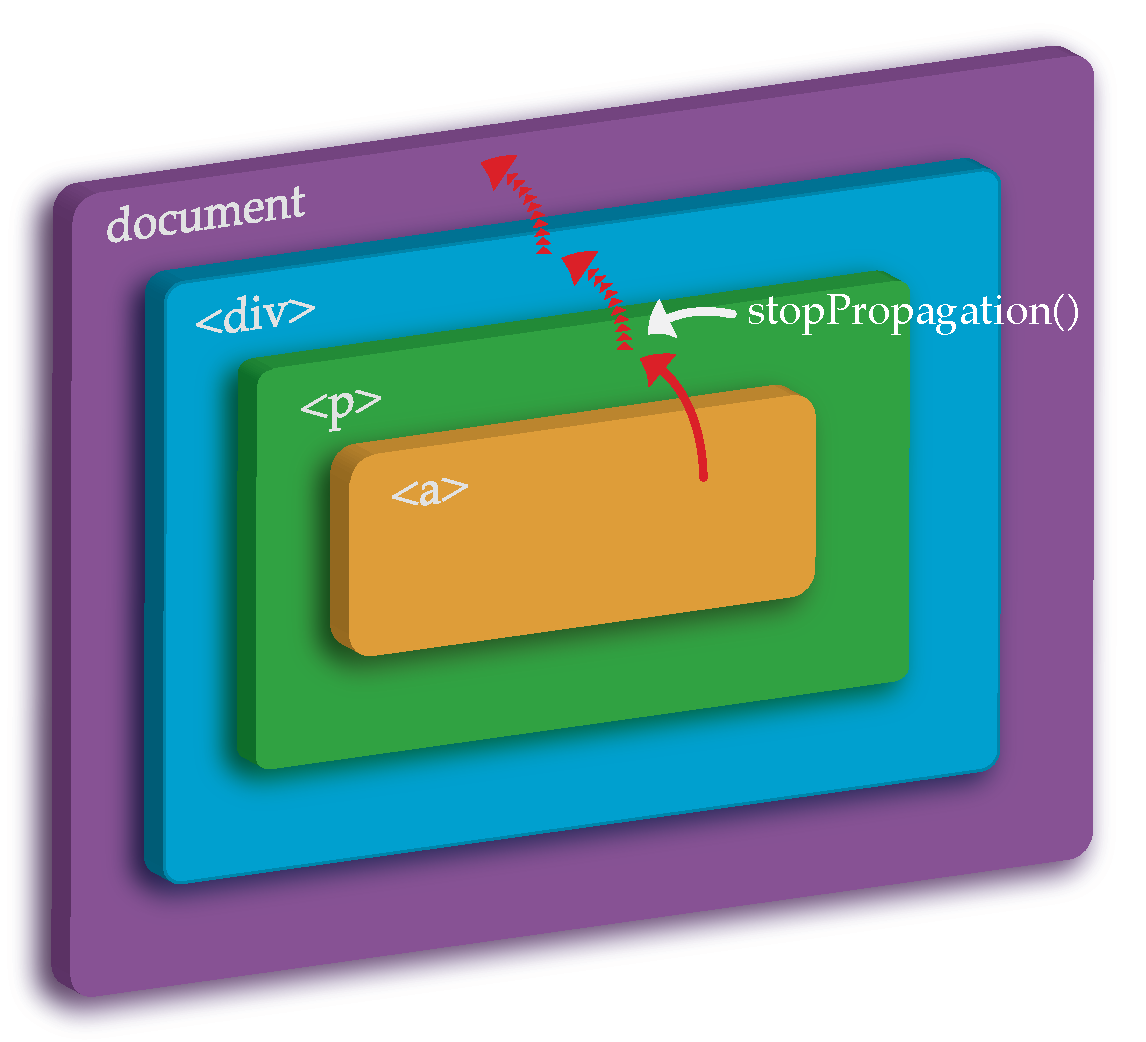
\includegraphics[width=\textwidth]{dom-event-bubbling}
  \caption[DOM event propagation]{DOM event propagation and the effect of stopPropagation()}
  \label{fig:dom-event}
\end{figure}

% subsubsection domobjects (end)

% subsection dom (end)
\subsection{AJAX} % (fold)
\label{sub:ajax}

Since its beginnings, the Web has been document based.
This means that, when the visitor wants more information and clicks on a link, the browser would request and load another whole document.
Even in web applications, the browser would have to reload the full page to send any information from the user and update the page.

\begin{wrapfigure}{r}{0.5\textwidth}
  \centering
    
\includegraphics[width=0.48\textwidth]{logo-not-ajax}
  \caption[AJAX logo]{This is not the \idx{AJAX} logo you are looking for}
  \label{fig:javascript-logo}
\end{wrapfigure}

This turns out to be inefficient and overkill in most situations, since web applications do not need to reload the full page in every user interaction but only update a little amount of information.
To address this problem several solutions where developed, from frames to applets, but they were too cumbersome or foreign respect the basic web technologies.

In 1999, \idx{Microsoft} proposed and implemented in its \idx{Internet Explorer} a new \idx{ActiveX} control to asynchronously load new data from the server without need to reload the page.
Using \idx{JavaScript}, that data could be requested on demand once the page was loaded, and through callbacks the data could be processed and the user interface changed accordingly.

Later, the rest of the browsers vendors implemented a similar technology under the \idx{XMLHttpRequest} object.
As this was gradually introduced, web developers started using it but it did not become a popular approach until 2004, when several big web applications such as \idx{Gmail} were developed.

Then, the term \ida{AJAX} was coined \cite{AJAX} to designate the technologies involved in the process, though most of them can be replaced by others while maintaining the same spirit.
Seeing how useful it had become, the \ida{W3C} decided to standardize the \idx{XMLHttpRequest} object.

As depicted in Figure~\ref{fig:ajax-application-model}, this approach needs another layer of complexity in the client to handle the data and update the interface.
This \ida{AJAX} engine means that much more \idx{JavaScript} code in the client is needed.
Eventually, this enables the rise of heavy web applications running in the client, with a substantial codebase to maintain and support across several browsers.

\begin{figure}[htbp]
  \centering
    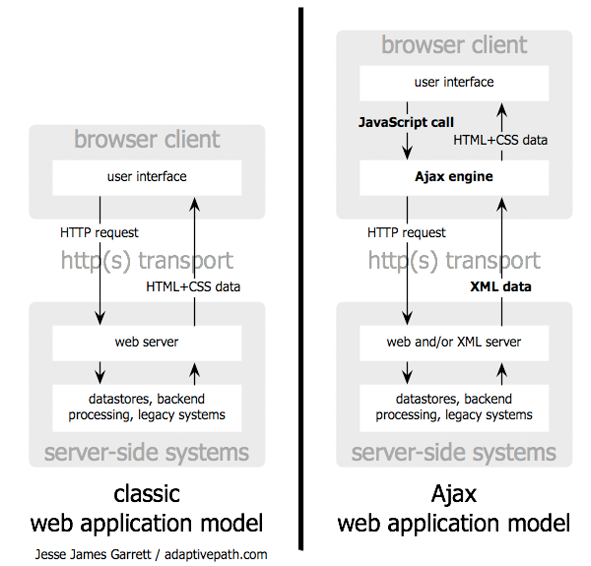
\includegraphics[width=\textwidth]{ajax-application-model}
  \caption[AJAX web application model]{AJAX web application model compared to the classic one.\newline© Jesse James Garrett}
  \label{fig:ajax-application-model}
\end{figure}

From the point of view of the user, the experience is much less disruptive than the classic model, as seen on Figure~\ref{fig:ajax-flow}.
When a user clicks a link or a button in a traditional web application, the user interface blocks, goes blank, and he has to wait until another page is fully reloaded if he wants to continue with another task.

\begin{figure}[htbp]
  \centering
    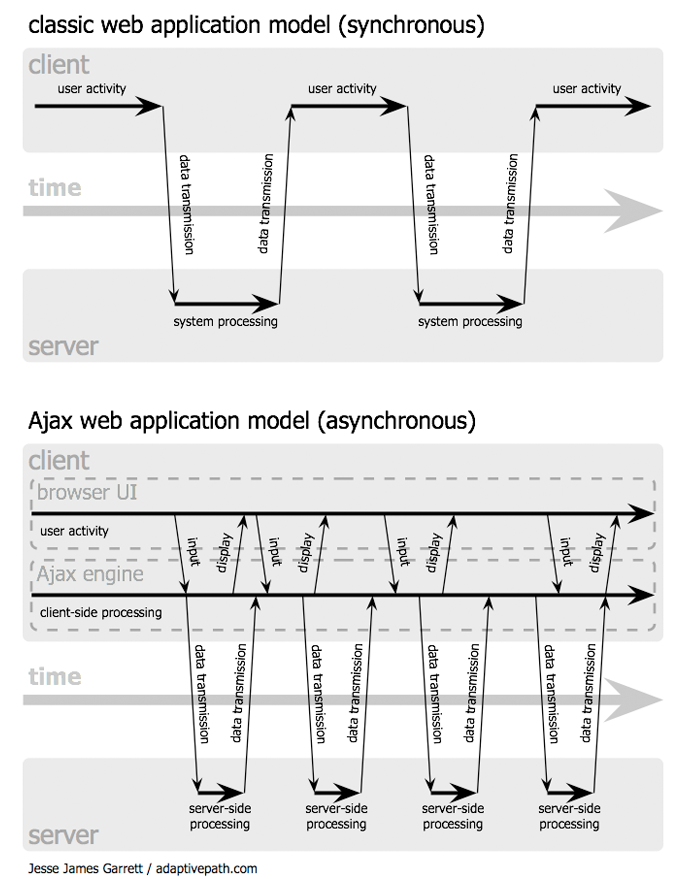
\includegraphics[width=\textwidth]{ajax-flow}
    \caption[AJAX flow]{Flow of the actions in a AJAX web application.\newline© Jesse James Garrett}
  \label{fig:ajax-flow}
\end{figure}

In an \idx{AJAX} application, when the user performs such actions, the interface does not block; instead the \idx{AJAX} engine is notified and the interface is \emph{instantly} available.
Meanwhile, backstage data gets interchanged and the client is updated, so that it can refresh the interface using the \ida{DOM} and a mix of \ida{HTML} and \ida{CSS}.

Though it could appear that the application has more overhead now, the user will notice a much more responsive application. Also, the requests should be much faster than before, since the browser does not need to process again all the resources or redraw the whole page, and the server only needs to generate fragments of data.

However, there are some drawbacks to this approach.
The first one is that the browser offers no feedback whatsoever to the user, but that is easily solved: the interface needs to reflect some visual feedback, like a spin ball.
The second one is that the application will break the history of the user, since no new page has been served, it cannot go back to the previous state or even link to it.
This has also been solved by the \ida{HTML}5 History \ida{API}, that allows to manipulate the browser history.

The third and hard one is that users with \idx{JavaScript} disabled will not be able to use this web application at all.
The best practice is to offer an alternate version with plain \ida{HTML} pages, but sometimes that is not possible or it makes no sense.
In the case of this project, since it was mostly experimental and not oriented for mainstream users, it was decided that such alternative would not be developed.

\subsubsection{How XMLHttpRequest works} % (fold)
\label{ssub:xmlhttprequest}

First of all, a \idx{XMLHttpRequest} object must be created, and a custom function that will be act as a callback must be set in its \texttt{onreadystatechange} property.
The next step consists of opening the connection to the server, with its \texttt{open()} method, specifying at least three parameters: first the \ida{HTTP} method to use (\texttt{"GET"} or \texttt{"POST"}), then the url that we wish to contact and finally if the requests should be asynchronous or not.
This last parameter is usually set to \texttt{true}, otherwise the user interface will block.

From now on, this object can make as many requests as it needs.
To make a request its \texttt{send()} method is used, with additional data if the method is \texttt{POST} or with no data (or \texttt{null}) if the method is \texttt{GET}.
Additionally, and only if needed, the \texttt{setRequestHeader()} method could be used to modify the headers of the \ida{HTTP} request.
If the request is asynchronous, the flow of the program will continue normally; if not, the program will block until the server sends all the data.

Some time later, the server will answer with the response data.
Then, the callback specified in the \texttt{onreadystatechange} property will be called, with all the needed data already updated in the \idx{XMLHttpRequest} object.
Actually, this callback will be called not only once but several times, each time reporting the progress of the request.
To be sure that the request was completed it is need to check that the \texttt{readyState} property is exactly 4, and to know that the requested resource is ok that the \texttt{status} property is 200 (this is the \ida{HTTP} state response).

If after that all was according to plan, the plain data will be accessible from the \texttt{reponseText} property.
Also, if the response is in \ida{XML}, the \texttt{reponseXML} property is also available with the parsed \ida{XML} tree (the reason of the X in \ida{AJAX}).
The callback will then usually make some \ida{DOM} manipulation to reflect the change in the interface.

Given the usefulness of this technique, most third-party libraries have implemented wrappers and more straightforward \ida{API}s to cover more use cases.
Also, there are different variations, for example the current trend is not to use the \ida{XML} format but to transmit everything in \ida{JSON}, a much more efficient markup language that is native to \idx{JavaScript}.

% subsubsection xmlhttprequest (end)

\subsubsection{JSONP} % (fold)
\label{ssub:jsonp}

By design, \idx{XMLHttpRequest} carries a severe restriction: it is only allowed to request \ida{URL}s from the same domain.
There are security reasons for this decision, but in this mashup golden era it hinders a lot of its purposes.
Thankfully, another technique has been popularized: \ida{JSONP}.
Less elegant than \ida{AJAX} but equally effective in most situations and without that ugly restriction.

The concept is simple and it is based on the fact that it is possible to add external scripts to a webpage.
Just add a \texttt{script} tag with the desired \ida{URL} and it will be executed; use the \ida{DOM} and that script can be dynamically added after the page is loaded, just like \ida{AJAX}.
Of course, that script must be written in \idx{JavaScript}, so that explains why  \ida{JSON} is used to pass the required data.

Listing~\ref{jsondata} shows how some data could be expressed in \ida{JSON} so that it can be used as an \ida{AJAX} response.
A question appears, how is that data going to be executed in order to access it?
The answer is by telling the external server to wrap it up in some function that we have define in our \idx{JavaScript} code.
The way to tell that to the other server is to add the name of the function to the requested \ida{URL} as a parameter (usually called \texttt{jsonCallback} or just \texttt{callback}).

\begin{lstlisting}[language=JavaScript,label=jsondata,caption=Some JSON data]
  {
    name:   "Kermit",
    animal: "Frog",
    age:    56,
    height: 45
  }
\end{lstlisting}

For example, if we tell the other server that the function is called \texttt{doSomethingWithData()}, it can then wrap it up in a way that the data is the parameter for that function (see Listing~\ref{jsonpdata}).
Since this code will be executed in our web application, it will call that function with that data at the exact moment the file is received and parsed.
Therefore, that function must be defined in the global object, so it can process the received data without any problem.

\begin{lstlisting}[language=JavaScript,label=jsonpdata,caption=Same JSON data wrapped in a custom function]
  doSomethingWithData({
    name:   "Kermit",
    animal: "Frog",
    age:    56,
    height: 45
  });
\end{lstlisting}

Obviously, the server must explicitly support this technique, otherwise it is impossible to receive and change the server response without the use of proxies.
Also, \ida{JSONP} should only be applied with trusted third parties, since any malicious code could be injected in the page.
The last security concern is that \texttt{POST} is not \emph{supported}, so any parameter has to be passed using \texttt{GET}, i.e., adding the parameters to the \ida{URL}.
However, due to its utility, almost all the popular libraries have similar tools that homogenizes  the use of \ida{AJAX} and \ida{JSONP}.

% subsubsection jsonp (end)

% subsection ajax (end)

% section javascript (end)
\section{JavaScript Framework: MooTools} % (fold)
\label{sec:mootools}

So far, \idx{JavaScript} seems a pretty powerful tool, focused on a limited scope but enough to make advanced web applications.
Sadly, in the real world additional tools are needed to obtain a certain level of productivity.
So let's briefly discuss why bringing yet another component to the application.

\subsection{Why Use a JavaScript Framework?} % (fold)
\label{sub:whymootools}

Most web application rely on \idx{JavaScript} frameworks, some are community driven efforts and others are custom made for an specific organization.
All of them have as first goal to reuse pieces of code in common tasks, something even more important in \idx{JavaScript} as it can be a very quirky language.
In our case, there are several reasons that lead to using a well-stablished framework:

\begin{itemize}
  \item Because we want to support different browsers.
  If we do not use a framework a lot of time would be spent debugging the \emph{huge} differences between \idx{Internet Explorer} and the rest of the browsers.
  Popular frameworks have been tested by thousands of developers, so it is less probable that we fall into a bug.
  \item Because we want to speed up the development.
  Usually these frameworks cover several holes in the \idx{JavaScript} specification that allows us fixing common issues with less code.
  Covering those holes by ourselves would be a waste of time, since in this project performance is not crucial.
  \item Because we want the interface to have advanced effects.
  We could just search for several scripts that makes one individual effect, but that will result in redundancies, differences in quality code and waste time in searching.
\end{itemize}

In the end, all of that means that we can focus on just writing our application, avoiding reinventing the wheel over and over.

% subsection whymootools (end)

\subsection{Making the Decision} % (fold)
\label{sub:decision}

By the previous standards, we have plenty of options to choose from:
\idx{jQuery}\footnote{\url{http://jquery.com/}},
\idx{Prototype}\footnote{\url{http://www.prototypejs.org/}},
\idx{Dojo}\footnote{\url{http://www.dojotoolkit.org/}},
\idx{YUI}\footnote{\url{http://developer.yahoo.com/yui/}},
\idx{GWT}\footnote{\url{http://code.google.com/webtoolkit/}},
\idx{Ext JS}\footnote{\url{http://www.extjs.com/}}, etc.
Overall, these are very popular and they offer high quality and plenty of functionality, while maintaining a similar performance.
However, for this particular project, and after some consideration, \idx{MooTools}\footnote{\url{http://mootools.net}} was considered the best option.
This decision was backed up by these reasons:

\begin{description}

  \item[Compact] It has a low footprint on the site load because it is reasonably lightweight for the functionality it offers.
  Particularly, it is more optimized in this aspect than \idx{Prototype}, \idx{YUI} or \idx{Dojo}, but then it was also slightly more compact than \idx{jQuery}.

  \item[Modular-Based] Because of that, the installation can be customized to get only the modules we need, and the creation of our own extensions is easier.

  \item[Compatible] It has been tested with most browsers: \idx{Internet Explorer} 6+, \idx{Firefox} 2+, \idx{Opera} 9+, \idx{Safari} 3+ and \idx{Chrome} 4+.

  \item[Functional] It offers all the functionality required for the first phase of the project: \idx{drag\et drop}, resizing, animations, etc.

  It also offers other functionality like \idas{AJAX} support, \idc{Hash} creation or \idc{Cookie} handling, that ease the development in different browsers.

  \item[Object-Oriented] By adding \emph{Classes} to \idx{JavaScript}, an abstraction that it is perfect for this application, since the server code is written is \idx{Java}.

  This way, we can use similar concepts both in the server and in the client.
  Moreover, the inherited code for \idx{ScaleNet} already used \idx{JavaScript} objects.

  \item[Extensive] It also has a repository for official plugins called  \idx{MooTools More} (with similar code quality and documentation to the \idx{MooTools Core}) and other third-party plugins can be found in the web.

  \item[Well-documented] It has extensive documentation for every class of the  framework.

  \item[Well-structured] Its structure is perfect for a professional web application.
  Frameworks like \idx{jQuery} are more focused in reducing the lines of code that in encouraging robust coding.\footnote{A MooTools developer further discussed this in: \url{http://jqueryvsmootools.com/}}
  \idx{MooTools} also helps reducing the lines of code, but it has more tools for writing code in a very modular, reusable and robust way, for example by using classes and other abstractions.

  It also improves the readability of the code, something hard to do in \idx{JavaScript}.
  Another important point of this framework is that it is based on prototype extensions (mainly \idc{DOM} extensions), so the syntax is very Object-Oriented and the code seems very clean.

  \item[Used by the \ac{APE} server\index{APE server}]
  So if we use that component, it will be very straightforward to write extensions in \idx{JavaScript} also in the server.
  This will mean that we could use the same coding style and the same tools in the server as in the client.

\end{description}

Previous experience with \idx{jQuery} resulted in quite faster development, but with time the solutions were hard to maintain without putting a lot of effort.
With \idx{MooTools}, several architectural design decisions like the use of \emph{Classes} and \emph{options} suited perfectly a non-trivial application like this one.

% subsection decision (end)

\subsection{MooTools Core} % (fold)
\label{sub:mootools_core}

The first thing to know about \idx{MooTools} is that works by \emph{monkey-patching} the native objects.
This means that it modifies the prototype of that objects and extends or changes its functionality.

Some experts consider this to be a very bad practice because code from different parties can easily collide.
However, this \idx{JavaScript} feature is very powerful and in good hands it turns out extremely convenient.
Due to this, it is very straightforward to write code with \idx{MooTools}, and the resulting code do not have to look different from raw \idx{JavaScript}.

Under some circumstances these extensions just patch native methods that are not available in all browsers so that the developer can use them avoiding compatibility headaches.
These additions are meaningfully named and can be organized into eight categories:

\begin{description}
  \item[Core] Traditionally \idx{MooTools} declared several utility functions in the global scope, but these have been deprecated in favor of equivalents methods in native objects.
  Last version (1.3) only keeps a handful of them, mostly for type checking and extending prototypes.
  \item[Types] Five important native types have been supercharged with a myriad of utility functions, filling a lot of holes in the \idx{JavaScript} specification: to deal with collections and iterators (\idc{Array}), to manipulate strings (\idc{String}) and numbers (\idc{Number}), to modify and custom call functions (\idc{Function}), to add information to events (\idc{Event}) and even to modify the properties in any object (\idc{Object}).
  \item[Browser] A new object (\idc{Browser}) is created with all the information about the browser and its environment conveniently organized.
  This not only includes the browser version, the installed plugins and the user platfom, but it also detects some key features.
  \item[Class] This is probably the heart of \idc{MooTools}.
  \idc{Class} is an object that encapsulates all the prototype-based inheritance system into the much more intelligible classic \ida{OOP}.
  Basically, a \idx{Class} is just an object with shortcuts to simulate traditional class inheritance and interface implementation.
  
\begin{lstlisting}[language=JavaScript,label=mootoolsclass,caption=MooTools class definitions]
  var Animal = new Class({
    Implements: [Options, Events],
    options: {
      name: "Unnamed",
      pace: 0,
      children: []
      // onWalk: $empty
    },
    initialize: function(options) {
      this.setOptions(options);
      if (this.options.pace > 10)
        this.fast = true;
    },
    walk: function(distance) {
      for (var i = 0; i < distance; i += this.pace) {
        this.fireEvent('onWalk', distance);
      }
    }
  });
  
  var Horse = new Class({
    Extends: Animal,
    initialize: function(options) {
      options.pace = 20;
      this.parent(options);
    }
  });
\end{lstlisting}
  
  This does not hide any good side effect of the prototype system, for example a class can be modified and extended in any time: it is as dynamic as any \idx{JavaScript} object.
  Simply, it is easier to use for a programmer that prototypes.
  
  On top of that, three powerful abstractions are built into the framework and appear in most other classes (that implement them):
  \begin{description}
    \item[Options] Handy way of dealing with settings within an \emph{instance}\footnote{Since everything is an object in \idx{JavaScript}, there are not really instances. In this context, an instance is an object cloned from a \idx{MooTools} class, usually with \texttt{new} statement defining particular values.}, that is, attributes that may be optional (non-optional attributes could be defined as plain properties).
    By using a \idc{Hash} to store all these properties, constructors only need one parameter to hold any combination of them.
    
    Because its options and the default values must be defined at the \emph{class declaration}, the framework can transparently merge both hashes.
    Therefore, since the developer does not need to handle this task anymore, it results in very clean constructors while resulting in a pretty extensible solution.
    \item[Events] The concept of a event is greatly stretched in \idx{MooTools}, as any class can define and fire custom events so that its instances can hook methods in the code of its parents.
    It integrates well with \idx{MooTools} options, so it is very easy to declare and use them.
    \item[Chain] This abstraction is designed to chain pieces of code to be executed asynchronously but in order.
    The usual example is to deal with animations in several steps, but it can be applied to a lot of different problems.
    Since \idx{JavaScript} is single-threaded but asynchronous by nature, it is very welcomed to have an alternate way to arrange chunks of code with a lower priority to the background while preserving certain order between them.
  \end{description}
  \item[Element] As any other good modern framework, \idx{MooTools} offers extensive support for \ida{DOM} manipulation.
  It has two global shortcut functions baked in: the dollar function \texttt{\$()} acts mostly as an alias for \texttt{document.getElementById()}, while \texttt{\$\$()} selects an array of \ida{DOM} elements based on the specified \ida{CSS} selector.
  
  These two functions returns objects of type \texttt{Element}: \ida{DOM} elements supercharged with utility extensions.
  For example, the constructor allows to quickly build an element with its own attributes, styles, size and events at once.
  Not only it is more expressive but it handles for us developers the differences between all supported browsers.
  \item[Fx] In the beginning, \idx{MooTools} was only a lightweight library to add visual effects, but with time it became a full-fledged framework.
  Consequently, it is no surprise to say that it has a very robust animation system in place.
  
  The base class is \texttt{Fx}, but normally developers should use \texttt{Fx.Tween} (to animate one property in an element) or \texttt{Fx.Morph} (to animate more than one property at the same time).
  There are also shortcut methods in \texttt{Element} for simple and quick animations.
  Apart from those classes, \texttt{Fx.Transitions} offers a broad collection of tweening transitions.
  \item[Request] An \ida{AJAX} wrapper that accumulates many options.
  There are subclasses to deal with \ida{HTML} and \ida{JSON} responses, and generally it takes a lot of work when setting \ida{AJAX} requests.
  For example, there are shortcuts in the \texttt{Element} class that with a simple one-line method can completely replace an element with a remote fragment.
  \item[Utilities] Four classes that have no place in previous categories: a cookie handler, a \ida{JSON} encoder/decoder, a \texttt{domready} event (that springs when the, ehem, \ida{DOM} is ready) and a Flash bridge (\texttt{Swiff}).
\end{description}

% subsection mootools_core (end)

\subsection{MooTools More} % (fold)
\label{sub:mootools_more}

In a separate package, official plugins outside of the previous categories have been compiled.
This includes advanced pieces of code that apply in too specific situations to be included in the main distribution, like form handling, interface widgets, advanced effects and other extras.
There are too many to be explained in this document, but the most important ones used in the project could be quickly enumerated:

\begin{description}
  \item[Class.Occlude] This class implements the singleton pattern, and ties the resulting object to a predefined \ida{DOM} element.
  \item[Hash] A simple hash implementation, with methods that make it more useful to hold collections than a simple \idx{JavaScript} objects.
  \item[Element.Position / Element.Measure] Handy wrappers that calculate the exact dimensions of an object.
  \item[Fx.Elements] To animate several elements at the same time.
  \item[Fx.Accordion] A visual effect suited to make room for several elements in a limited space: as one element expands, the others gradually collapse.
  \item[Fx.Move] Another visual effect to move an element from one location to another.
  Positions need not to be defined in coordinates, they can rather be automatically calculated from target elements.
  \item[Drag / Drag.Move] To easily add drag\et{}drop capabilities, making use of events to treat all possible outcomes.
  It also offers shortcuts to make an element automatically draggable and/or resizable.
  \item[Request.JSONP] Similar class to \texttt{Request}, but using the \ida{JSONP} technique to retrieve remote data from other domains.
  \item[Assets] To dynamically load scripts, stylesheets, images and other resources.
  \item[Hash.Cookie] This class handles the creation of a cookie that will contain a plain hash.
\end{description}

% subsection mootools_more (end)

% section mootools (end)

\section{Push Server: the APE Server\index{APE server}} % (fold)
\label{sec:ape}

Because of technical limitations of traditional browsers, it is not trivial to develop real time applications with \idx{JavaScript}.
More precisely, since it cannot directly push data from the server to the browser, the only native solution is to poll in regular time intervals --- an inefficient approach.

The apprehended solution in the old system was to embed a \idx{Java} applet solely to communicate with the server.
The \idx{Java} \ida{API} for applets includes support for sockets, so it is possible to pass data in real time.
However, the big drawback is that it needs the \idx{Java} plugin to be installed in browsers, and there is no plugin for mobile browsers --- neither in \idx{iOS} nor in \idx{Android}.

It was decided that mobile browsers must be supported by the second iteration of this project, so a new solution native to those browsers should be considered, getting rid of this \idx{Java} applet.

\subsection{Comet} % (fold)
\label{sub:comet}

Shortly after \ida{AJAX} was popularized, another technique ---called in contrast \idx{Comet}--- was developed to solve the particular use case of pushing data from the server to the client.
Since then, several alternatives for creating real-time applications have been developed:

\begin{figure}[htbp]
  \centering
    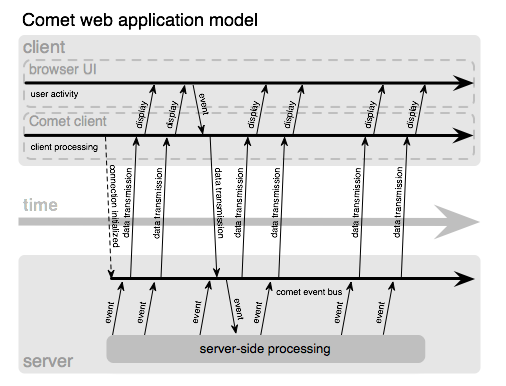
\includegraphics[width=\textwidth]{comet-flow}
  \caption[Comet flow]{Typical flow in a Comet application (compare with Figure~\ref{fig:ajax-flow})\newline© Alex Russell / \url{infrequently.org})}
  \label{fig:comet-flow}
\end{figure}

\begin{description}
  \item[\idx{WebSocket} \ida{API}] An \ida{HTML}5 extension\footnote{\url{http://dev.w3.org/html5/websockets/}} easy to use that just offers a socket to any server.
  This would be the perfect choice (and it should be chosen in the future), but at the moment it severely lacks support among the supported browsers, so it cannot be considered.
  \item[\idx{Socket.IO}] Since real sockets in browsers are out of the equation, an application with both browser and server components is the only way to go.
  One of the options with a brighter future relies on \idx{NodeJS}\footnote{\url{http://nodejs.org/}}, an effort to bring \idx{JavaScript} to the server.
  
  \idx{Socket.IO}\footnote{\url{http://socket.io/}} is a simple software that simulates real sockets in the browsers and uses \idx{NodeJS} for its server component.
  It holds quite interesting ideas, but it was discarded because then it was in a pretty immature state.
  \item[\idx{CometD}] This is a similar approach by the \idx{Dojo} Foundation\footnote{\url{http://cometd.org/}} (so it works well with the dojo framework), creating a new protocol called Bayeux\footnote{\url{http://svn.cometd.com/trunk/bayeux/bayeux.html}}.
  In a quick glance it was rejected because it seems too complex for this task, and it could end in adding an additional framework in the mix.
  \item[\ac{APE} server\index{APE server}] And finally we get to the winner of our contest.
  The \ida{APE} project\footnote{\url{http://www.ape-project.org/}} is a solid full solution with two components (server/browser), and it is focused on supporting real time data streaming.
  Just visiting its website explains why it seems like a better solution, because of the extensive documentation and well-explained examples --- from simple to advanced ones.
  
  One of the reasons why it was chosen it that it offers many layers of tinkering.
  If we only want a socket to a existing server, it has a proxy socket built so it is not needed to write any additional server code.
  But if we need to develop an advanced application, custom modules for the server can be written in \idx{JavaScript}.
  
  The other big reason is that it is written with \idx{MooTools}, so bringing \ida{APE} to the table bears little overhead for the client code.
  In the server, a hypothetical custom module could benefit from having the same framework as in the browser.
\end{description}

After considering all options, the \ida{APE} project looked the most promising one.
Eventually, just the proxy socket was needed, so it was merely a drop-in replacement for the \idx{Java} applet.
In any case, as its server deployment (see \S\ref{sec:apeconfig}) consists on almost exclusively installing the \idx{Debian} \ida{APE} package, it results in an elegant and painless solution.

% subsection comet (end)

\subsection{How the APE Server Works} % (fold)
\label{sub:how_the_ape_server_works}

As we said, the system needs two components: one to be installed in the server and a script to be included in our web application.
The first component is a typical web server that listens upon a port, with the special peculiarity that only understands the \ida{APE} protocol.

\begin{wrapfigure}{r}{0.5\textwidth}
  \centering
    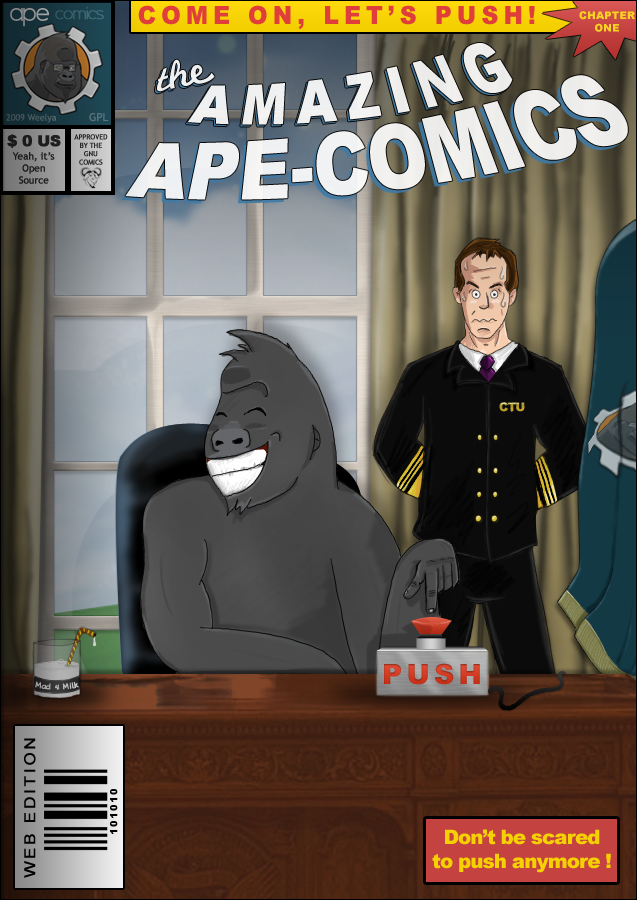
\includegraphics[width=0.48\textwidth]{ape-comic}
  \caption{Real official APE documentation}
  \label{fig:ape-comic}
\end{wrapfigure}

In that server, modules can be written in \idx{JavaScript} (or even \idx{C}), with a convenient \ida{API} to access common web resources like sockets, pipes or \idx{MySQL} connections.
There are some modules and plugins implemented by default, like one that acts as a proxy for \ida{TCP} sockets, or other that redirects data from a server application to the client.
With those two simple modules a lot of applications can be written without needing a custom module.

The server maintains a list of named channels; each channel holds one or more users that can write and read from that channel.
Again, every user can have more than one connection, for example a user that has two tabs open in the same browser, or that have two sessions in two different devices at the same time.
For this, the server \ida{DNS} must be configured to answer to multiple dynamic subdomains  (\verb|1.ape.domain.com|, \verb|2.ape.domain.com|, \verb|42.ape.domain.com|, etc).

In the browser, a set of scripts must be added to our web application so that they can talk with the backend: the \ac{APE} \ac{JSF}\index{APE JSF}.
The configuration is very basic: it only needs the \ida{URL} for the rest of the scripts and the base domain of the \ac{APE} server\index{APE server}.

Then the \ida{APE} client can be created, the connection opens and the two parties start exchanging messages.
Messages are formatted as \ida{JSON} arrays that contains two groups of objects: \emph{commands} and \emph{raws}.
The former ones come from browsers to the server while the latter ones go the other way around.

Commands should be taken as actions that the clients want to accomplish, like opening the connection or sending some data.
Commands are composed by a name, a challenging number (increased each time, to numerate the messages) and optional parameters.
Depending on the name, the message is processed by the very \ac{APE} server\index{APE server} or served to a custom module that will answer to that action.

Raws can be expressed as data sent by the server, indeed it is composed by a name, a timestamp and the data as a \ida{JSON} object.
Again, the name reveals the purpose of the transmission and the data format.
It is not uncommon for a message (that is, a \ida{JSON} array) to contain more than one raw.

To send a command, the client creates a \idc{GET} or \idc{POST} request to a increasingly numerated subdomain, encoding the \ida{JSON} array as the only parameter.
When there is data to send, the server answers and the raw(s) can be found in the body response.

% subsection how_the_ape_server_works (end)

\subsection{Transport Methods} % (fold)
\label{sub:transport_methods}

Though it is not completely essential to know how exactly the \ac{APE} server\index{APE server} works in the backend, it should be understood how it earns its push capabilities.
There are four transport methods implemented that the developer can choose from, but each of them has its strengths and weaknesses.

\begin{description}
  \item[\idx{Long-polling}] This is the default transport method (so it will be selected unless noted otherwise), and it works in pretty much every \idx{JavaScript}-enabled browser.
  It is based on \ida{AJAX} but with a twist: the client request a resource but the server keeps the \ida{HTTP} connection open until it has something to say.
  
  When there is data to send (or after a certain timeout), the server sends the response.
  Then, the client immediately re-request the same resource, so the server has always a connection open to the browser.
  Of course, the main drawback of this approach is that it is more like a hack, so it could be done more efficiently.
  \item[\ida{JSONP}] Similar to the previous one but over \ida{JSONP} instead of \ida{AJAX}, so it offers cross-domain possibilities.
  \item[\idx{XHRStreaming}] Also very similar to the first one, with the exception that the server do not close the connection when it has information to send.
  Therefore it only needs one connection, so it is more efficient.
  Sadly, this only works with recent browsers.
  \item[\idx{WebSockets}] As said before, this only works in a few new browsers, so it does not make sense to support it just yet if most times it is going to fallback to the default transport method.
\end{description}

% subsection transport_methods (end)

TODO: this goes in chapter3

\begin{lstlisting}[language=JavaScript,label=apesocket,caption=TCPSocket usage in APE JSF]
var client = new APE.Client();
var socket;

client.load();
client.addEvent('load', function() {
  this.core.start();
});

client.addEvent('ready', function() {
  socket = new this.core.TCPSocket();
  socket.open(host, port);
  socket.onopen = function() {
    socket.send('hello world');
  };
  socket.onread = function(msg) {
    console.log('New message: ' + msg);
  };
  socket.onclose = function() {
    socket = null;
    console.log('Connection with the server closed.');
  };
}

window.addEvent('unload', function() {
  socket.close();
}
\end{lstlisting}

% section ape (end)

\section{Mobile Web Development} % (fold)
\label{sec:mobile}

Lorem ipsum dolor sit amet, consectetur adipisicing elit, sed do eiusmod tempor incididunt ut labore et dolore magna aliqua. Ut enim ad minim veniam, quis nostrud exercitation ullamco laboris nisi ut aliquip ex ea commodo consequat. Duis aute irure dolor in reprehenderit in voluptate velit esse cillum dolore eu fugiat nulla pariatur. Excepteur sint occaecat cupidatat non proident, sunt in culpa qui officia deserunt mollit anim id est laborum.

\subsection{Touchscreens} % (fold)
\label{sub:touchscreens}

Lorem ipsum dolor sit amet, consectetur adipisicing elit, sed do eiusmod tempor incididunt ut labore et dolore magna aliqua. Ut enim ad minim veniam, quis nostrud exercitation ullamco laboris nisi ut aliquip ex ea commodo consequat. Duis aute irure dolor in reprehenderit in voluptate velit esse cillum dolore eu fugiat nulla pariatur. Excepteur sint occaecat cupidatat non proident, sunt in culpa qui officia deserunt mollit anim id est laborum.

% subsection touchscreens (end)

\subsection{Webkit} % (fold)
\label{sub:webkit}

Lorem ipsum dolor sit amet, consectetur adipisicing elit, sed do eiusmod tempor incididunt ut labore et dolore magna aliqua. Ut enim ad minim veniam, quis nostrud exercitation ullamco laboris nisi ut aliquip ex ea commodo consequat. Duis aute irure dolor in reprehenderit in voluptate velit esse cillum dolore eu fugiat nulla pariatur. Excepteur sint occaecat cupidatat non proident, sunt in culpa qui officia deserunt mollit anim id est laborum.

% subsection webkit (end)

% section mobile (end)

% chapter stateoftheart (end)
